% ----------------------------  START --------------------------- 
\documentclass[../main]{subfiles} % main refers to main.tex
\graphicspath{{\subfix{../Illustrations}}}
\begin{document}
\addto\extrasfrench{\protected\edef:{\unexpanded\expandafter{:}}}
\selectlanguage{french}
% --------------------------------------------------------------- 

\begin{figure}[ht]
    \centering
    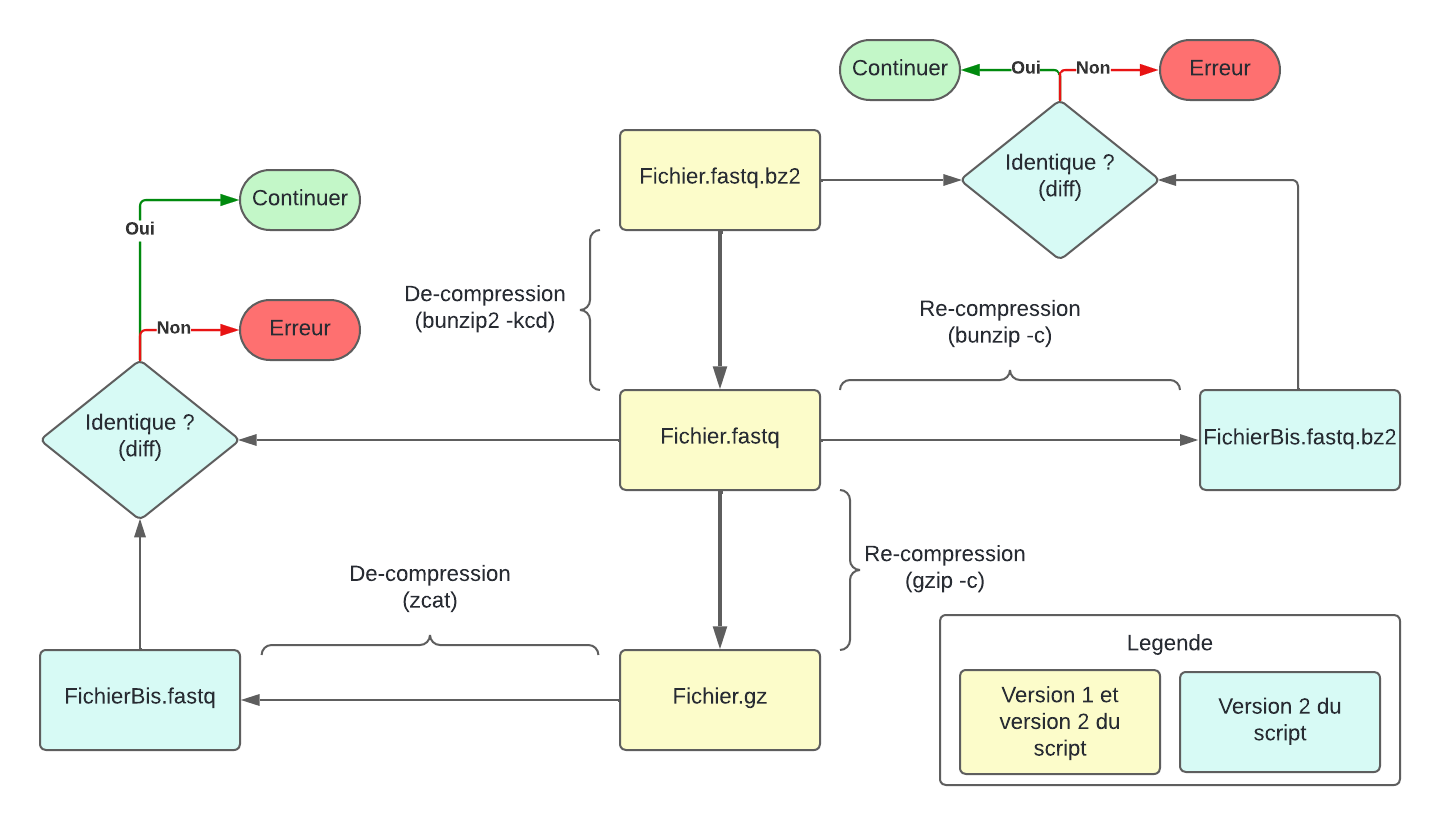
\includegraphics[width=0.9\textwidth]{../Illustrations/Decompression.png}
    \caption{Fonctionnement du programme de changement de compression des \fastq. Les cadres jaunes représentent les étapes communes à la version 1 et à la version 2 tandis que les cadres bleus représentent les étapes spécifiques à la version 2. Le programme est accessible ici : \cite{florent_f-marchalm1bioinfointernship2024-inrae_agap_ge2pop_2024}. Image faite avec \gls{Lucidchart}.}
    \label{fig:DiagDecompresse}
\end{figure}


% --------------------------------------------------------------- 
\end{document}
% ----------------------------  END --------------------------- 
